\documentclass{article}
\usepackage{tikz}
\usetikzlibrary{positioning,shapes}
\begin{document}
\title{A Letter to the Secretary of the Treasury}
\author{Mark Twain}
\date{Riverdale-on-the-Hudson, October 15, 1902}
\maketitle

\begin{quotation}
  \em
  This document consists of three versions:
  \begin{description}
  \item[uppercase:] the salutation is in uppercase.
  \item[nobonds:] the salutation is in uppercase, and the paragraph
    about government bonds omitted.
  \item[default:] the salutation is in small caps, and the paragraph
    about government bonds included.
  \end{description}
  There are also updated versions of all three documents, which
  include the description of the Riverdale.  The update is done in the
  nobonds version, and then propagated to the other versions of the
  document.  This is shown on Figure~\ref{fig:flow}.

  This document' version is 
nobonds.

This document is not updated.
\end{quotation}

\begin{figure}
  \centering
  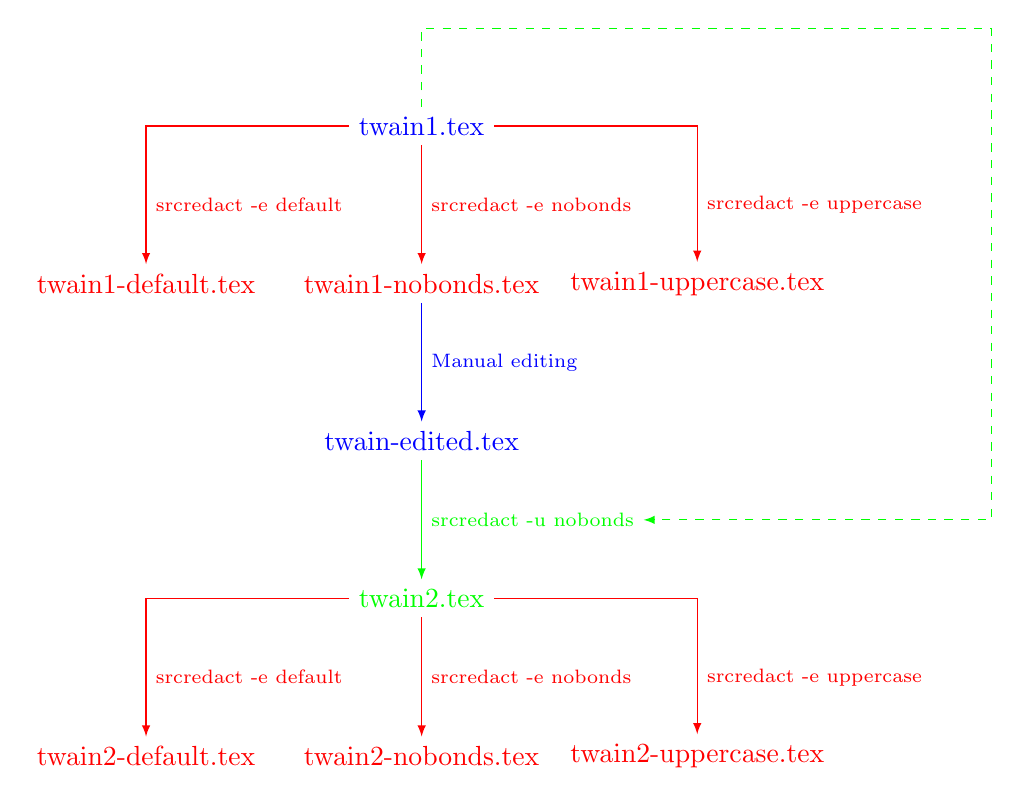
\begin{tikzpicture}
    \node[on grid] (twain1) {\color{blue}twain1.tex};     
    \node[on grid, below= 2cm of twain1] (twain1-nobonds)
    {\color{red}twain1-nobonds.tex};
    \node[on grid, left= 3.5cm of twain1-nobonds] (twain1-default)
    {\color{red}twain1-default.tex}; 
    \node[on grid, right= 3.5cm of twain1-nobonds] (twain1-uppercase)
    {\color{red}twain1-uppercase.tex}; 
    \node[on grid, below= 2cm of twain1-nobonds] (twainedited)
    {\color{blue}twain-edited.tex}; 
    \node[on grid, below= 2cm of twainedited] (twain2)
    {\color{green}twain2.tex}; 
    \node[on grid, below= 2cm of twain2] (twain2-nobonds)
    {\color{red}twain2-nobonds.tex};
    \node[on grid, left= 3.5cm of twain2-nobonds] (twain2-default)
    {\color{red}twain2-default.tex}; 
    \node[on grid, right= 3.5cm of twain2-nobonds] (twain2-uppercase)
    {\color{red}twain2-uppercase.tex}; 
    \draw[arrows=-latex, color=red] (twain1) -| 
    node[below=1cm, right] {\scriptsize srcredact -e default}
    (twain1-default); 
    \draw[arrows=-latex, color=red] (twain1) -- node[right]
    {\scriptsize srcredact -e nobonds} (twain1-nobonds);
    \draw[arrows=-latex, color=red] (twain1) -| 
    node[below=1cm, right] {\scriptsize srcredact -e uppercase}
    (twain1-uppercase); 
    \draw[arrows=-latex, color=blue] (twain1-nobonds) -- node[right]
    {\scriptsize Manual editing} (twainedited);
    \draw[arrows=-latex, color=green] (twainedited) -- node[right]
    (unredact) {\scriptsize srcredact -u nobonds} (twain2);
    \coordinate[above=of twain1] (above1);
    \coordinate[right=2 cm of twain1-uppercase] (right-uppercase);
    \draw[arrows=-latex, color=green, style=dashed] (twain1)
    -- (above1) -| (right-uppercase) |- (unredact);
    \draw[arrows=-latex, color=red] (twain2) -| 
    node[below=1cm, right] {\scriptsize srcredact -e default}
    (twain2-default); 
    \draw[arrows=-latex, color=red] (twain2) -- node[right]
    {\scriptsize srcredact -e nobonds} (twain2-nobonds);
    \draw[arrows=-latex, color=red] (twain2) -| 
    node[below=1cm, right] {\scriptsize srcredact -e uppercase}
    (twain2-uppercase); 
  \end{tikzpicture}
  \caption{Document workflow.  \textcolor{blue}{Blue}---manual edits,
    \textcolor{red}{Red}---generated by srcredact in extract mode,
    \textcolor{green}{Green}---generated by srcredact in unextract mode.}
  \label{fig:flow}
\end{figure}

THE HON. THE SECRETARY OF THE TREASURY, WASHINGTON, D.~C.:

Sir,---Prices for the customary kinds of winter fuel having reached an
altitude which puts them out of the reach of literary persons in
straitened circumstances, I desire to place with you the following order:


Twelve tons early greenbacks, range size, suitable for cooking.

Eight barrels seasoned 25 and 50 cent postal currency, vintage of 1866,
eligible for kindlings.

Please deliver with all convenient despatch at my house in Riverdale at
lowest rates for spot cash, and send bill to

Your obliged servant,

Mark Twain, Who will be very grateful, and will vote right.
\end{document}
